The main controls layer is in charge of processing and sending out the majority of the signals on the Turing Board. It uses the Jetson TX2 to communicate with the microprocessor in the wheels and turning layer to control the wheels and turning mechanism. There are several sensors in the wheels and turning layer that send information via the microprocessor to the Jetson as inputs. The Jetson also receives inputs from the power layer to know how much power is left in the battery. The last input to the Jetson comes from the Human Machine Interface (HMI) layer. This layer consists of items used to allow the Turing Board to understand the world around it and operate more appropriately. Along with the human machine interface layer, the computer vision layer also contributes to the Jetson TX2 receiving feedback from its environment. The computer vision layer uses RGB imagery and stereo and infrared imagery to see obstacles and the user depending on the mode it is currently in. Finally, the remote control for the Turing Board allows the user to control the board as an electric longboard when in the respective mode. The app boasts many features including user authentication and ride data analysis.

%%%%%%%%%%%%%%%%%%%%%%%%%%%%%%%%%%%%%%%%%%%%%%%%%%%%%%%%%%%%%%%%%%%%%%%%%%%%%%%%%%%%%%%%%%%%%
% If you want to change the image, put your image in the images folder and change "data_flow" 
% to the name of your image. You can also change the caption (System architecture) to 
% something else if you want.
\begin{figure}[h!]
	\centering
 	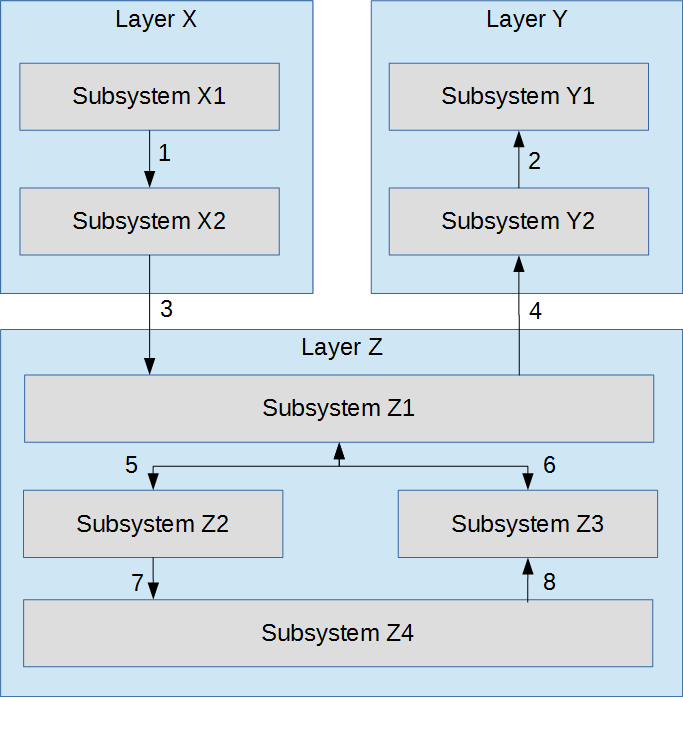
\includegraphics[width=0.90\textwidth]{images/data_flow} % Change me
 \caption{System Architecture}
\end{figure}
